        \documentclass[12pt] {article}
        \usepackage{amsmath}
        \usepackage[margin=0.5in]{geometry}
        \usepackage{pdfpages}
        \begin{document}

        \begin{flushright}
        Assignment No.: 1\\
        Name: Yuk Hang Terence Lai\\
        Student No.: 1000583362\\
        \end{flushright}

        \subsection*{Excercise 1}
        \bigskip
		\subsection*{Task 1:}

        \begin{flushleft}
        Important Notations Used:\\
        -$\rho_{* \rightarrow *1}(A)$: rename all attributes in table A to its attrute name with 1 appended to the end\\
        eg: $ \rho_{* \rightarrow *1}[A(name, date,time)]\implies  A(name1, date1, time1)$\\
        -$R \leftarrow$ (RA Expression): R is the final result for the question, assume it is the finished query for the question\\
        -Number beside each RA expression corrosponds to the comment below 
        \end{flushleft}


        Q1)
        \begin{align}
        	A &\leftarrow \Pi_{PID, CID}(\rho_{playerA, court  \rightarrow PID, CID }(Event)) \cup \Pi_{PID, CID}(\rho_{playerB, court  \rightarrow PID, CID}(Event))\\
        	B &\leftarrow \Pi_{CID}(Court)\\
        	C &\leftarrow \Pi_{PID}(A) - \Pi_{PID}((\Pi_{PID}(A) \times B) - A)\\
        	R &\leftarrow \Pi_{fname, lname}(\sigma_{name=Canada}(\rho_{country \rightarrow CTRYID}(C \bowtie Player) \bowtie Country))
        \end{align}
        \begin{flushleft}
        (1) Renaming the court attribute to CID, and rename PlayerA and playerB to a common attribute Consolidates PLayerA and PlayerB into a single attribute\\
        (2) Get the CID attribute from Court\\
        (3) Preform the equivelant of a A/B to get PIDs who played on all courts\\
        (4) Join with Player and Country and get only Player from canada then get their names\\
        \end{flushleft}

        Q2)
        \begin{align}
        	A &\leftarrow \rho_{event \rightarrow EID}(\Pi_{dateIssued, event}(Voucher))\\
       		R &\leftarrow \Pi_{dateIssued, date}(A \bowtie Event)
        \end{align}
        \begin{flushleft}
        (5) Get the dateIssued out of each voucher and the event it belongs to rename The event attribute to join with Event Table\\
        (6) Join with Event to get the date of the event and project\\
        \end{flushleft}

        Q3) \\
        
        	Not Representable\\
        
        Q4)
        \begin{align}
        	A &\leftarrow \Pi_{PID}(\rho_{playerA \rightarrow PID}(Event)) \cup \Pi_{PID}(\rho_{playerB\rightarrow PID}(Event))\\
        	B &\leftarrow [Player - (A \bowtie Player)]\\
        	R &\leftarrow \Pi_{name}(\rho_{country \rightarrow CTRYID}(B) \bowtie Country)
        \end{align}
        \begin{flushleft}
        (7) Get consolidated players from playerA and playerB attributes. This relation contains players who participated in at least 1 event\\
        (8) Join A (Players who have 1 event) with Player to get full tuple and subtract from Player to get Players who didn't play in an event\\
        (9) Join with Country and project the country name
        \end{flushleft}
        
        Q5) 
        \begin{align}
        	A &\leftarrow \sigma_{court = court1 \wedge EID \neq EID1}( Events \times (\rho_{* \rightarrow *1}(Events))) \\
            R &\leftarrow \Pi_{name, CID}((\rho_{court \rightarrow CID }(\Pi_{court}(Events)- \Pi_{court}(A))) \bowtie Court)
        \end{align}
        \begin{flushleft}
        (10) A contains all the Events where A court is used for more than 1 event (Different EID's but Same CID)\\
        (11) Subtract A from all events will return Courts with only 1 Event played on them. Join with court and project its CID and name
        \end{flushleft}
        
        Q6)\\

        define: 
        \begin{flalign*}
        d &= |setswonA - setswonB|\\
        d1 &= |setswonA1 - setswonB1|
        \end{flalign*}
        \begin{align}
        	A &\leftarrow \Pi_{setswonA, setswonB}(Event) - \Pi_{setswonA, setswonB}[\sigma_{d1 > d}(Event \times \rho_{* \rightarrow *1}(Event))]\\
        	B &\leftarrow A \bowtie Events\\
        	C &\leftarrow \Pi_{PID}(\rho_{playerA \rightarrow PID}(B)) \cup \Pi_{PID}(\rho_{playerB\rightarrow PID}(B))\\
        	R &\leftarrow \Pi_{name}(C \bowtie Player \bowtie \rho_{CTRYID \rightarrow country}(Country))
        \end{align}
        \begin{flushleft}
        (12) Get setswonA and setsWonB where the absolute difference between the 2 is the maximum\\
        (13) Get the events where these sets were recorded\\
        (14) Consolidate PlayerA and PlayerB attributes and Extract their PID info\\
        (15) Join PID with Player and Country and report the name of the country
        \end{flushleft}

        Q7)
        \begin{align}
        	A &\leftarrow \Pi_{capacity}(Court) - \Pi_{capacity}(\sigma_{capacity1 > capacity}(Court \times \rho_{* \rightarrow *1}(Court)))\\
        	B &\leftarrow [A \bowtie Court] \bowtie (\rho_{court \rightarrow CID}(Event))\\
        	R &\leftarrow \Pi_{PID}(\rho_{playerA \rightarrow PID}(B)) \cup \Pi_{PID}(\rho_{playerB\rightarrow PID}(B))
        \end{align}
        \begin{flushleft}
        (16) Get the court with the largest capacity\\
        (17) Get the events that were played in the largest court\\
        (18) Consolidate PlayerA and PlayerB attributes and Extract their PID info
        \end{flushleft}

        Q8)
        \begin{align}
            A &\leftarrow \Pi_{dateIssued}(Voucher) - \Pi_{dateIssued}(\sigma_{dateIssued1<dateIssued}(Voucher \times \rho_{* \rightarrow *1}(Voucher)))\\
    		B &\leftarrow (\rho_{event \rightarrow EID}(A \bowtie Voucher)) \bowtie Event\\
    		C &\leftarrow \rho_{playerA \rightarrow PID}(\Pi_{playerA}[\sigma_{SetswonA > SetswonB}(B)]) \cup 
    		\rho_{playerB \rightarrow PID}(\Pi_{playerB}[\sigma_{SetswonA < SetswonB}(B)])\\
    		R &\leftarrow \Pi_{name}(C \bowtie Player \bowtie \rho_{CTRYID \rightarrow country}(Country))
        \end{align}
        \begin{flushleft}
        (19) Get the minimum dateIssued value implying the earliest purchased voucher\\
        (20) Get the Event that Voucher was related to\\
        (21) Get the winning player of that event. The select is Mutually Exclusive, one set is always empty (as it selects the losing Attribute in the event)\\
        (22) Get the country of the winning player
        \end{flushleft}

        Q9) \\

        	Not Representable\\
        
        Q10)
        \begin{align}
        	A &\leftarrow \Pi_{EID, dateIssued, date, VID}(\rho_{event \rightarrow EID}(Voucher) \bowtie Event)\\
        	B &\leftarrow   \sigma_{dateIssued = date}(A) \bowtie \sigma_{dateIssued1 = date1}(\rho_{dateIssued, VID, date \rightarrow dateIssued1, VID1, date1}(A))\\
        	R &\leftarrow \Pi_{EID}(\sigma_{VID1 \neq VID}(B))
        \end{align}
        \begin{flushleft}
        (23) Join Voucher and Event together and project date and dateIssued for comparision, EID as the final output of the query, and VID as a Key \\
        (24) Find at least 2 instances where dateIssued = date \\
        (25) Use VID to remove the duplicate (Where the 2 joined Together have the same VID) and project the EID
        \end{flushleft}

        Q11)
        \begin{align}
        	A &\leftarrow \Pi_{wins}(Player)- \Pi_{wins}(\sigma_{wins1 > wins \wedge country1 = country}(Player \times \rho_{* \rightarrow *1}(Player)))\\
        	B &\leftarrow (\sigma_{wins \neq 0}(A)) \bowtie Player\\
        	R &\leftarrow  \Pi_{fname, lname, name}(B \bowtie \rho_{CTRYID \rightarrow country}(Country))
        \end{align}
        \begin{flushleft}
      	(26) Get the Max number of wins for each country (comparisons where countries are not matching will not be valid)\\
      	(27) Remove all entries with 0 wins (since 0 can be a max if all players of that country did not win). Join to get player data again\\
      	(28) Join with country and report the first name, last name and name of country
        \end{flushleft}

        Q12)
        \begin{align}
        	PA' &\leftarrow \Pi_{PID, CID, TID}(\rho_{playerA, court, tournament  \rightarrow PID, CID, TID }(Event))\\
        	PB' &\leftarrow \Pi_{PID, CID, TID}(\rho_{playerB, court, tournament  \rightarrow PID, CID, TID}(Event))\\
        	A' &\leftarrow  (PA')\cup(PB') \\
        	A &\leftarrow \Pi_{PID, CID}(A')\\
        	B &\leftarrow \Pi_{CID}(Court)\\
        	C &\leftarrow \Pi_{PID}(A) - \Pi_{PID}((\Pi_{PID}(A) \times B) - A)\\
        	D &\leftarrow \Pi_{slam, PID}((C \bowtie A') \bowtie Tournament)\\
        	E &\leftarrow \Pi_{slam}(Tournament)\\
        	F &\leftarrow \Pi_{PID}(D) - \Pi_{PID}((\Pi_{PID}(D) \times E) - D)\\
        	R &\leftarrow \Pi_{globalRank}(F \bowtie Player)
        \end{align}
        \begin{flushleft}
        (29) Rename playerA court and tournament\\
        (30) Rename playerB court and tournament\\
        (31) Consolidates PlayerA and PlayerB into a single attribute Along with CID and TID added to the relation. Represents which player has played on what court and is in which tournament. \\
        (32) To Set up for division We only need PID, CID \\
        (33) Get the CID attribute from Court\\
        (34) Preform the equivelant of a A/B to get PIDs who played on all courts\\
        (35) Join C back with A' and join with tournament to get slam info. Relation represents which player has played in which slam that is confirmed to play in all courts \\
        (36) Get the slam attribute from Tournament\\
        (37) Preform the equivelant of a D/E to get PIDs who played on all slams\\
        (38) Join with Player and report the global rank 
        \end{flushleft}

        \subsection*{Task 2:}
        \begin{flushleft}
        Q1) $\sigma_{playerA = playerB}(Event) = \emptyset$\\
        \bigskip
        Q2) $ A \leftarrow \Pi_{PID, date}(\rho_{playerA \rightarrow PID}(Event)) \cup \Pi_{PID, date}(\rho_{playerB\rightarrow PID}(Event))$\\
        $\sigma_{date < activeSince}(A \bowtie Player) = \emptyset$
        \bigskip
        Q3) $\sigma_{eventdate - dateissued < 10000}(\rho_{event \rightarrow EID}(Voucher) \bowtie (Event)) = \emptyset$\\
        \bigskip
        Q4) Cannot be expressed\\
        \bigskip
        Q5) $\sigma_{slam \neq AO \wedge slam \neq FO \wedge slam \neq UO \wedge slam \neq W }(Tournament) = \emptyset$\\
        \bigskip
        Q6) $ A \leftarrow \Pi_{PID, tournament}(\rho_{playerA \rightarrow PID}(Event)) \cup \Pi_{PID, tournament}(\rho_{playerB\rightarrow PID}(Event))$\\
        $\sigma_{gender \neq discipline}(\rho_{tournament \rightarrow TID}(A) \bowtie Tournament \bowtie Player) = \emptyset$\\
        \bigskip
        Relation A  represents which player has played in each event and the additional information related to that event.\\
        \end{flushleft}

        \subsection*{Excercise 2:}
        \bigskip
        \subsection*{Task 1:}
        \bigskip
        \begin{flushleft}
        a) Min Basis $= AB \rightarrow D, C \rightarrow E, D \rightarrow C, E \rightarrow A $\\
        b) Min Basis $= A \rightarrow D, BD \rightarrow E, AC \rightarrow E, DE \rightarrow B$\\
        c) Min Basis $= AB \rightarrow D, AC \rightarrow E, BC \rightarrow D, D \rightarrow A, E \rightarrow B$\\
        \end{flushleft}
        \medskip
        \subsection*{Task 2:}
        \begin{flushleft}
        Note: the *** represents a violation\\
        a)\\
        $AB^{+} = {ABCD}$\\
        ***$C^{+} = {CDA}$\\
        ***$D^{+} = {DA}$\\
        $R_{1} = CDA$\\
        $R_{2} = CB$\\
        \medskip
        FD's in $R_{1} = C \rightarrow D, D \rightarrow A, C \rightarrow A $\\
        $C^{+} = CDA$\\
        ***$D^{+} = DA$\\
        $R_{3} = DA$\\
        $R_{4} = DC$\\
        Final Relations:\\
        $R_{2} = CB$\\
        $R_{3} = DA$\\
        $R_{4} = DC$
        \end{flushleft}
        \begin{flushleft}
        b)\\
        $AB^{+} = ABCD$\\
        $BC^{+} = BCDA$\\
        $CD^{+} = CDAB$\\
        $AD^{+} = ADBC$

        No Violations, Final Relation:
        $R = ABCD$
       	\end{flushleft}
       	\begin{flushleft}
       	c)\\
       	\end{flushleft}
       	\begin{flushleft}
       	d)\\
       	$AB^{+} = ABCDE$\\
       	***$C^{+} = CDBE$\\
       	$R_{1} = CDBE$\\
       	$R_{2} = CA$\\
       	\medskip
       	FD's in $R_{1} = C \rightarrow D, D \rightarrow B, D \rightarrow E, C \rightarrow B, C \rightarrow E $\\
       	$C^{+} = CDBE$\\
       	***$D^{+} = DBE$\\
       	$R_{3} = DBE$\\
       	$R_{4} = DC$\\

       	Final Relations:\\
       	$R_{4} = DC$\\
       	$R_{3} = DBE$\\
       	$R_{2} = CA$

       	\subsection*{Excercise 3 diagrams below}

       	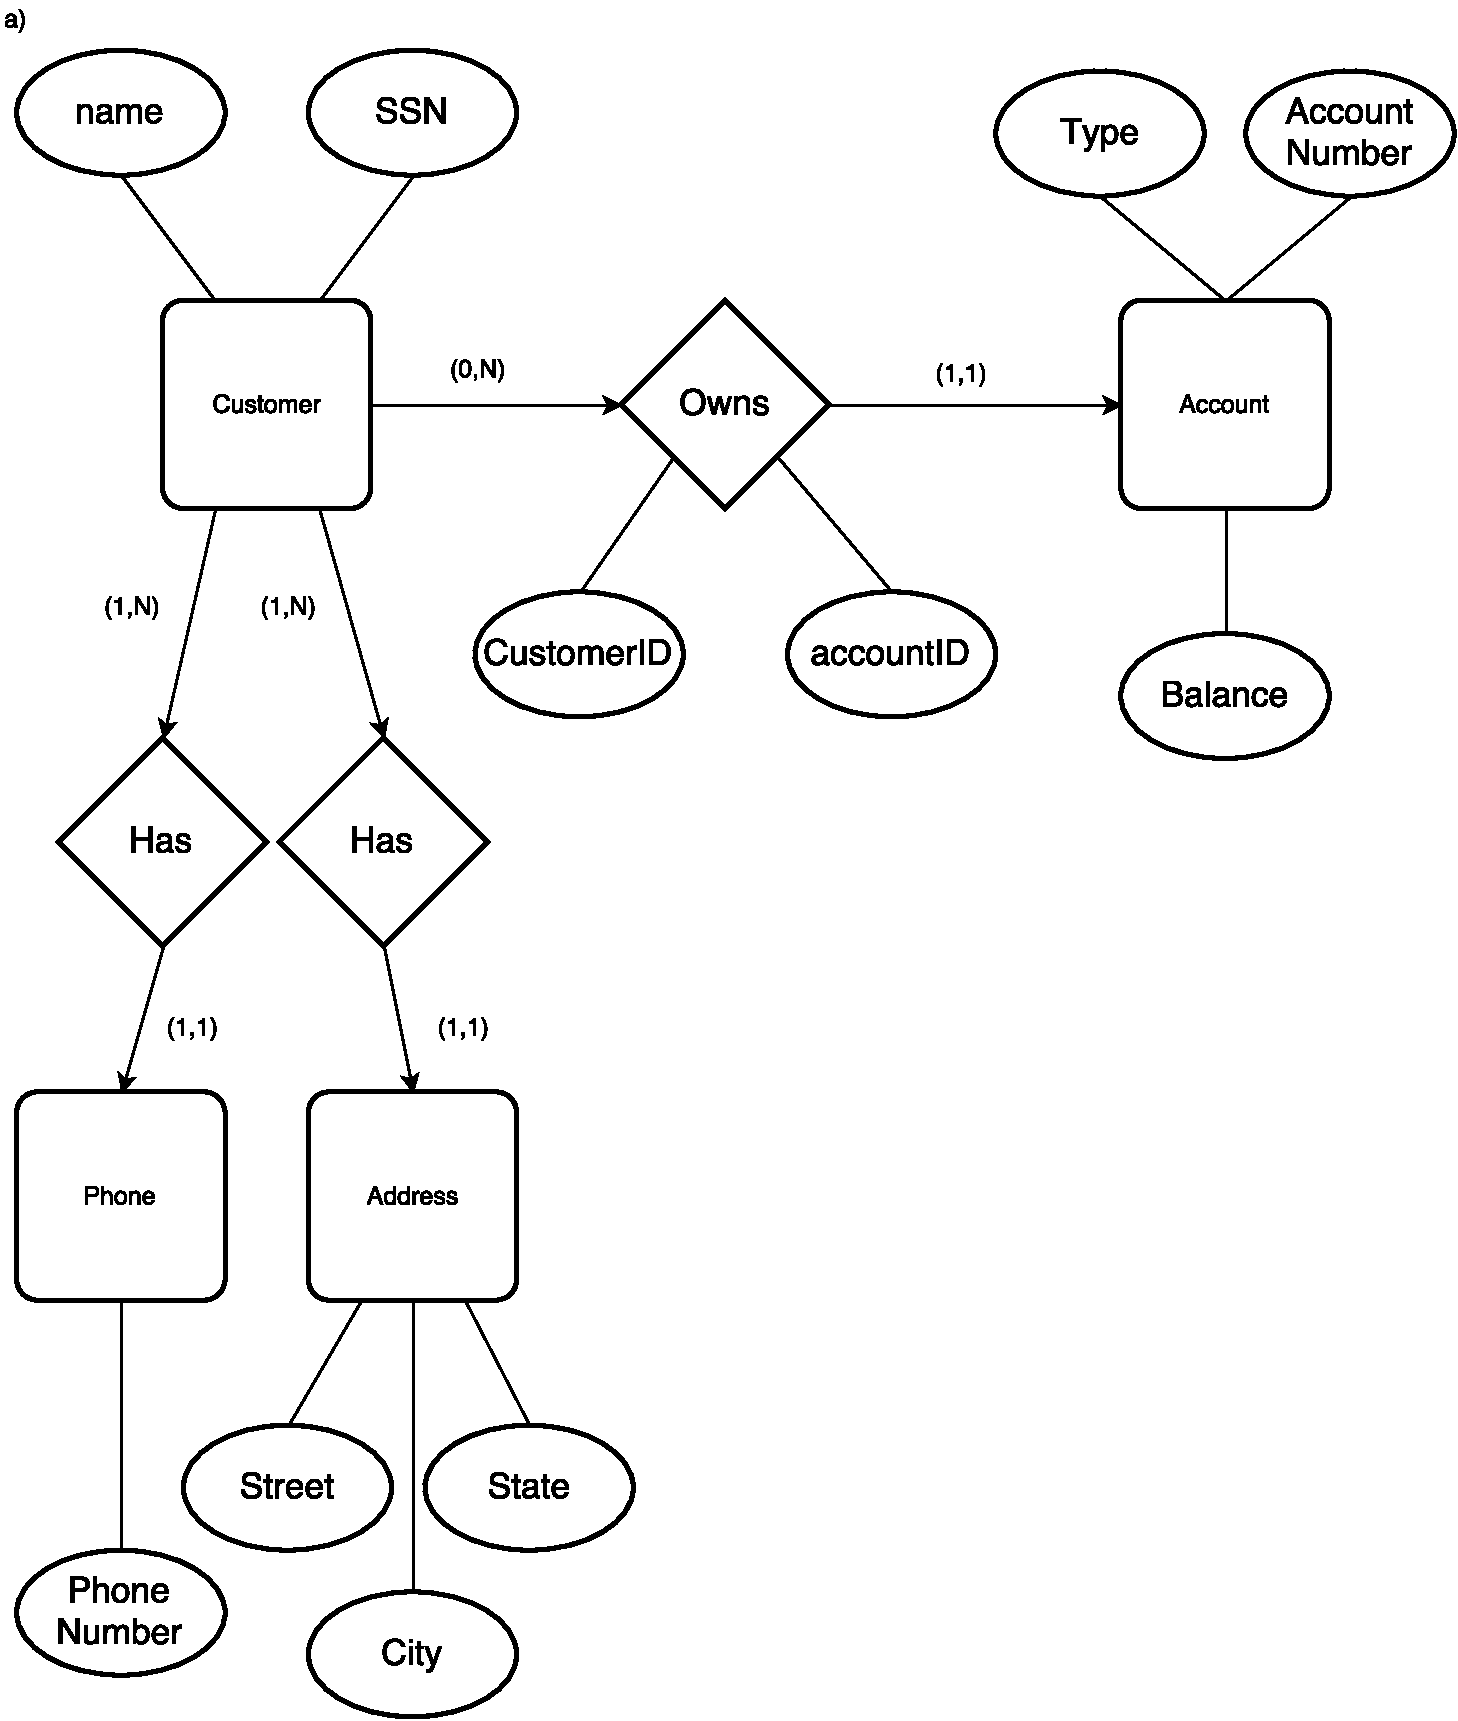
\includepdf[pages={1}]{/Users/Terence/git_repo/personal/diagrams/EX3T1P1.pdf}
       	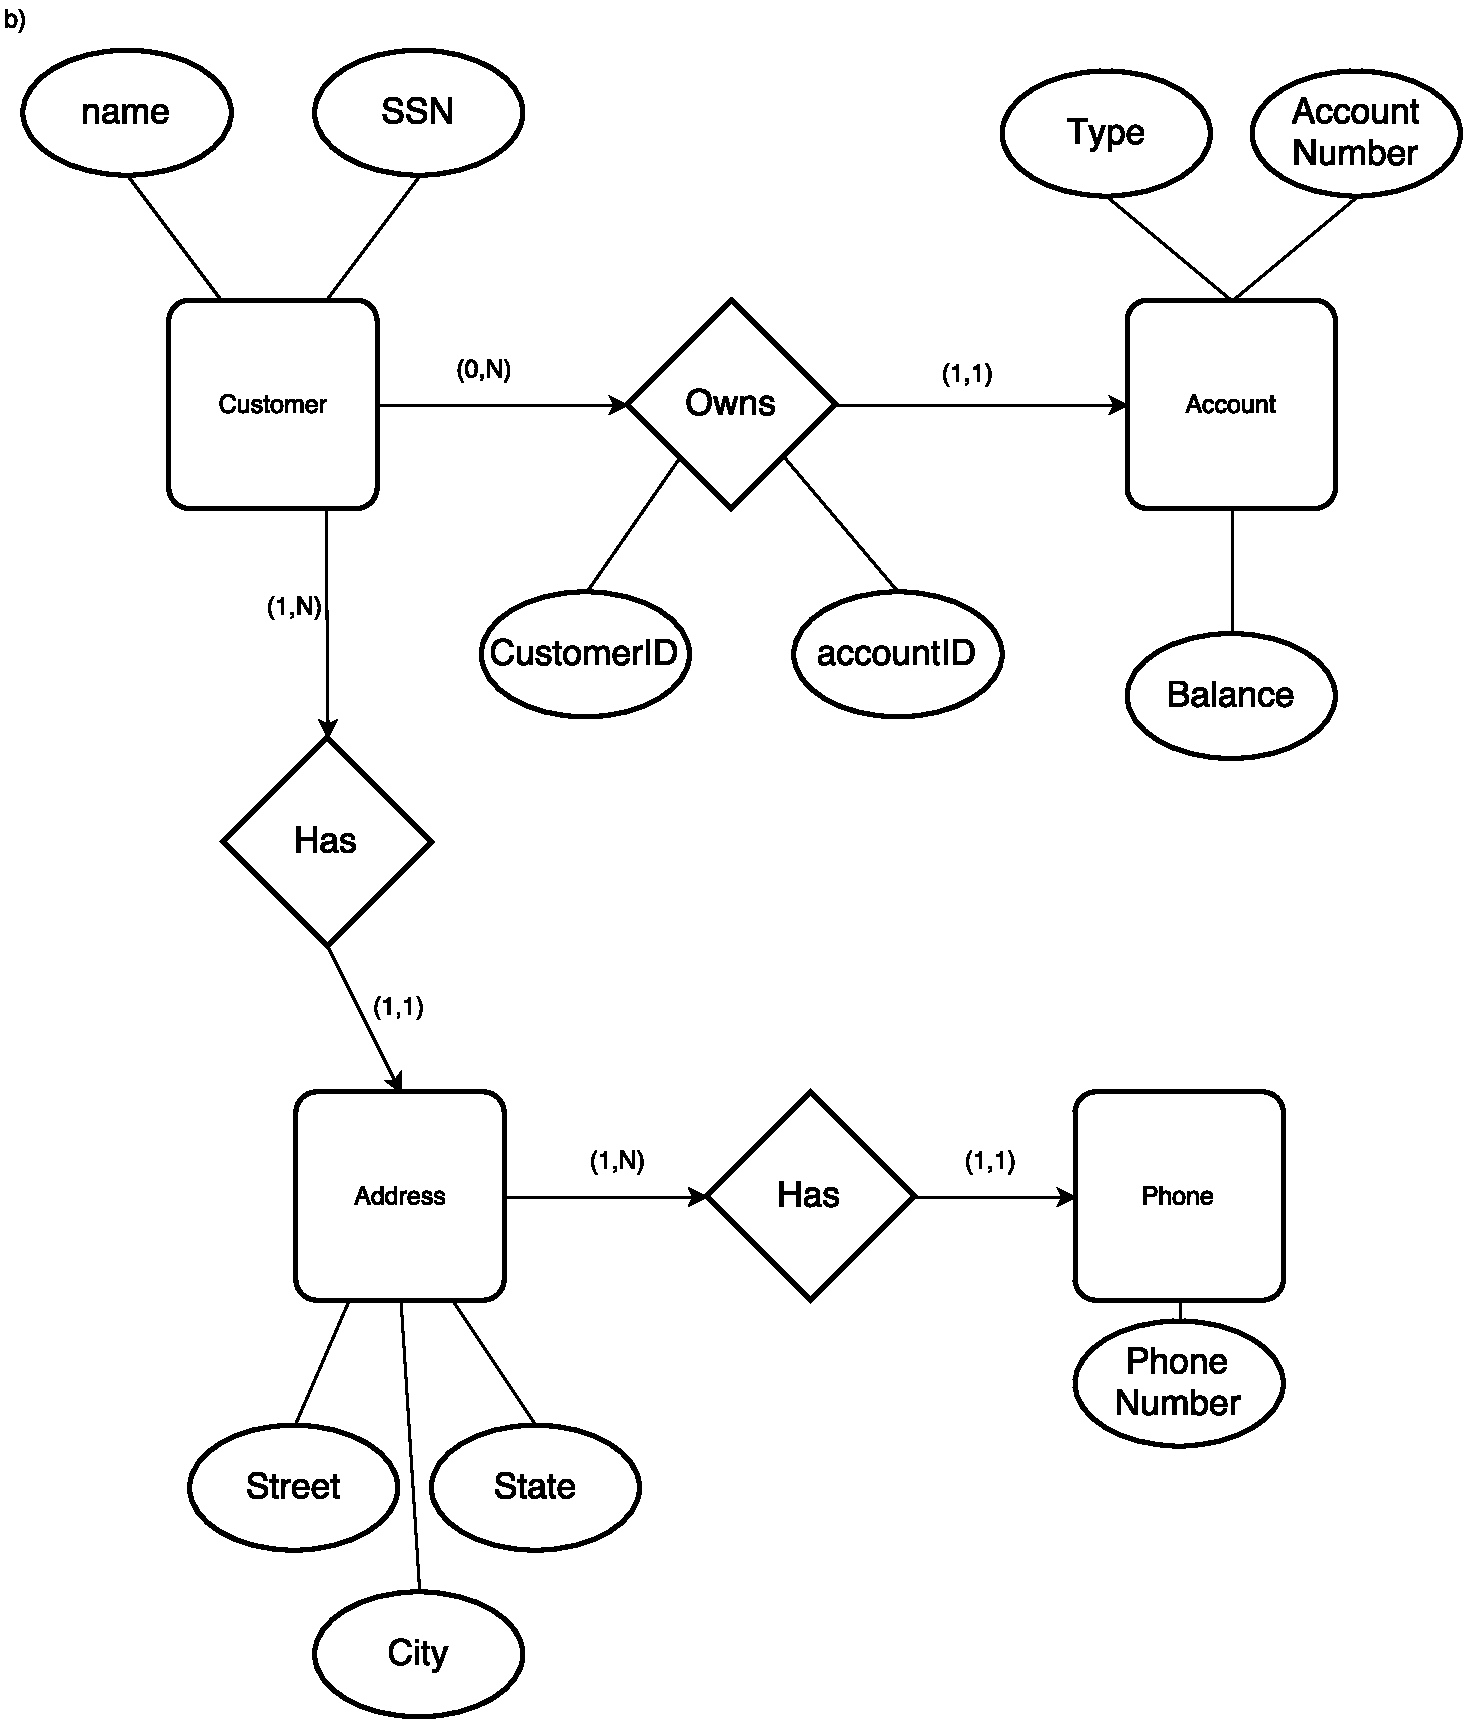
\includepdf[pages={1}]{/Users/Terence/git_repo/personal/diagrams/EX3T1P2.pdf}
       	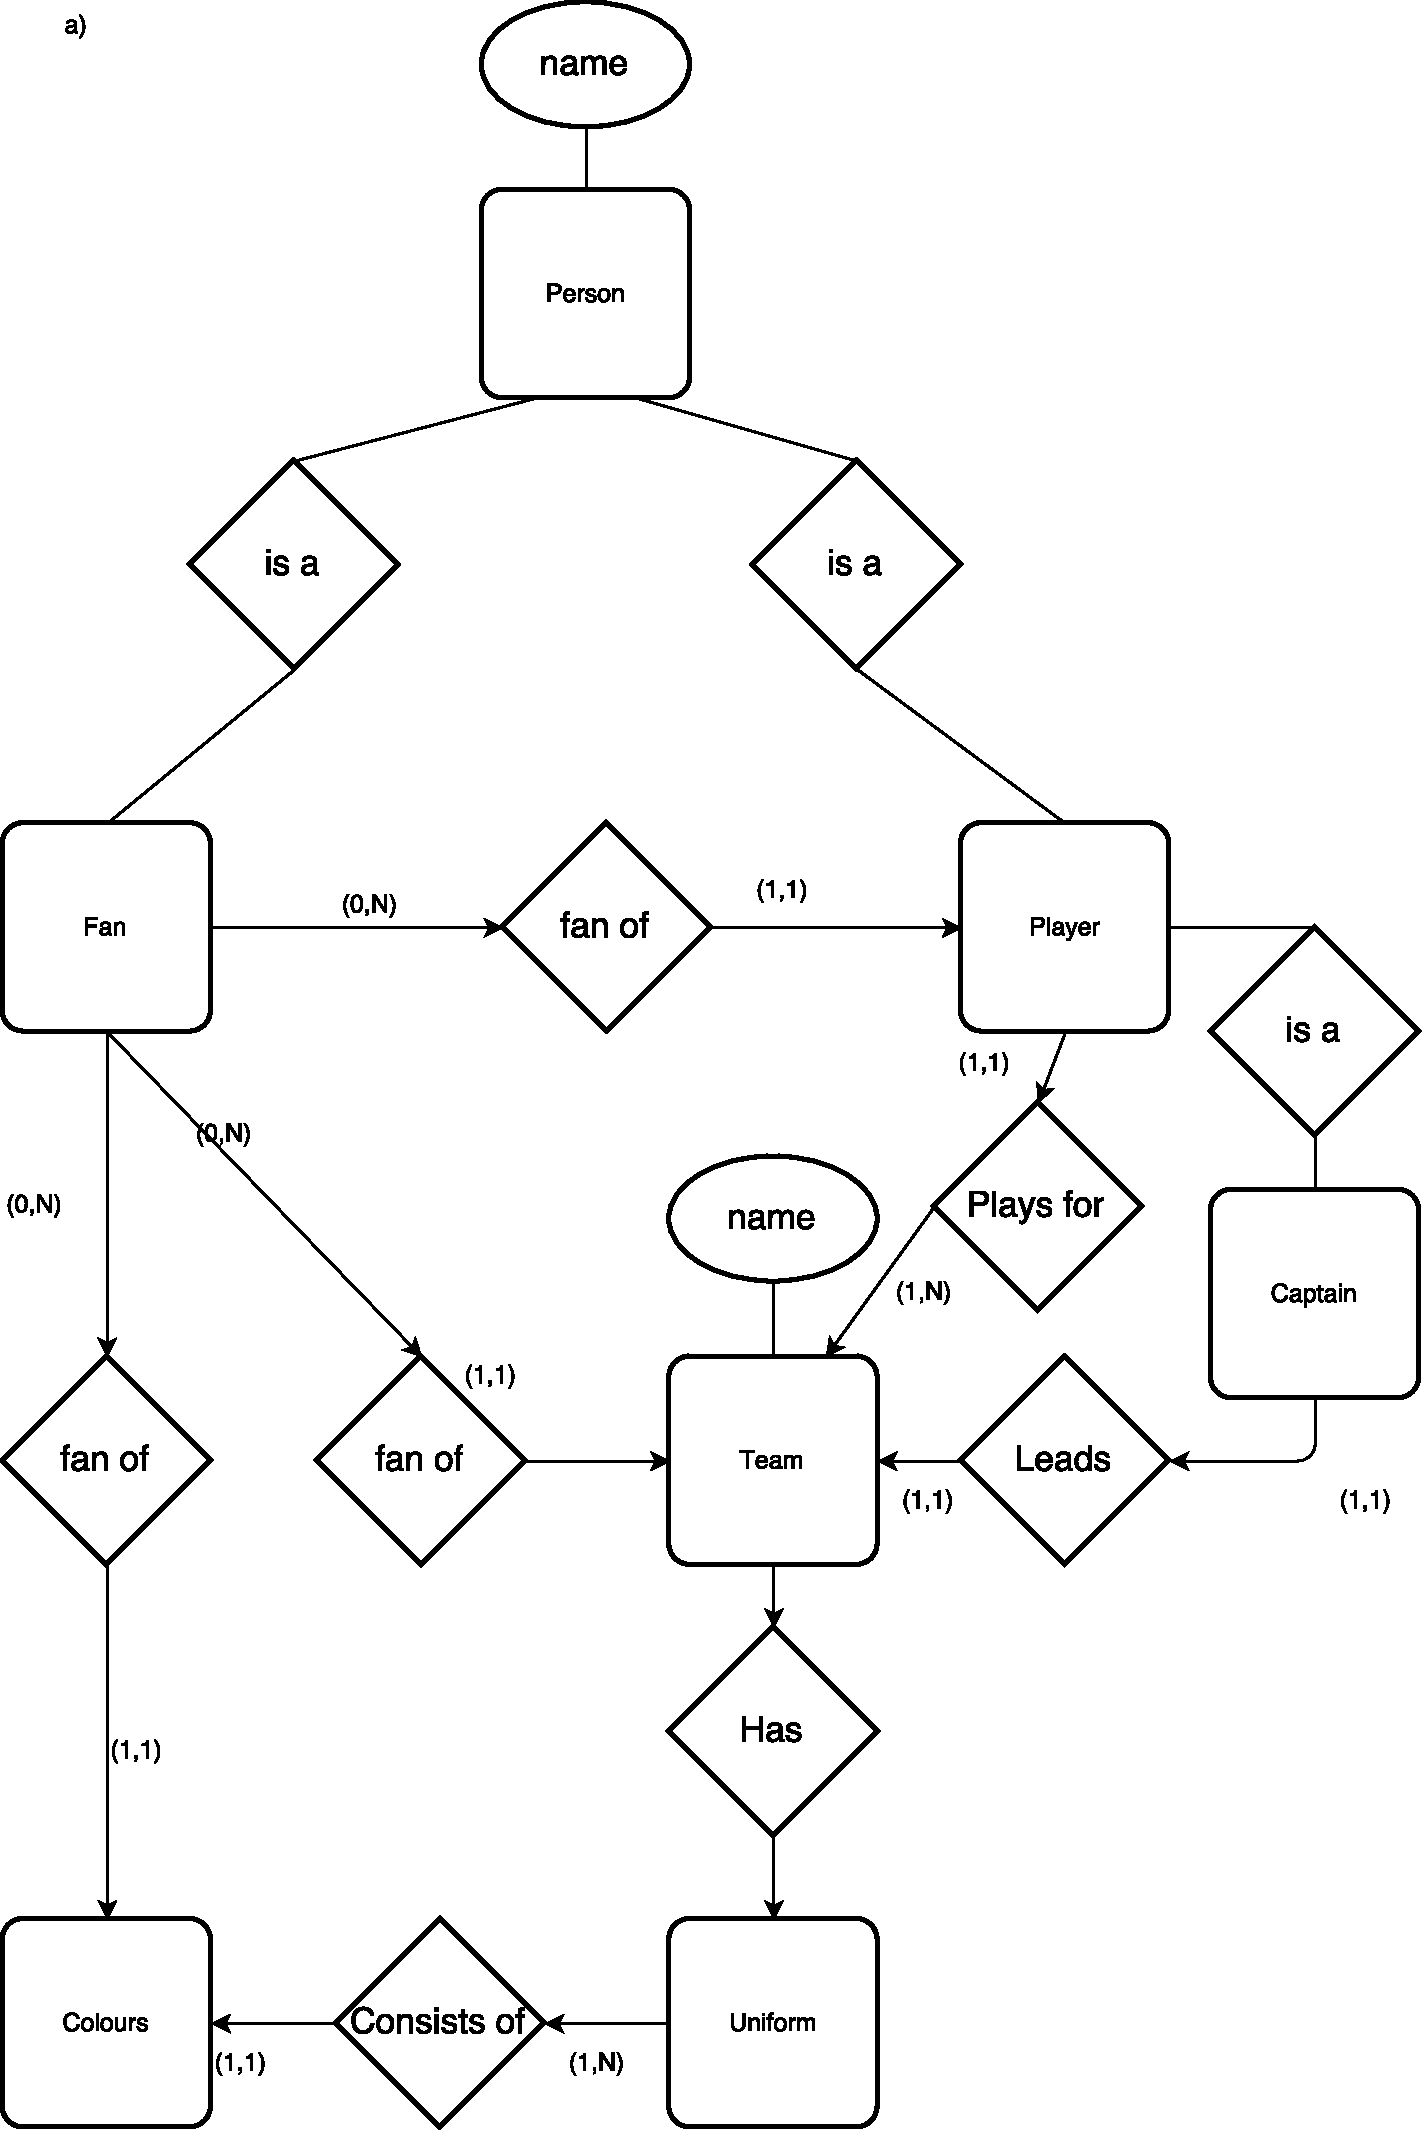
\includepdf[pages={1}]{/Users/Terence/git_repo/personal/diagrams/EX3T2P1.pdf}
       	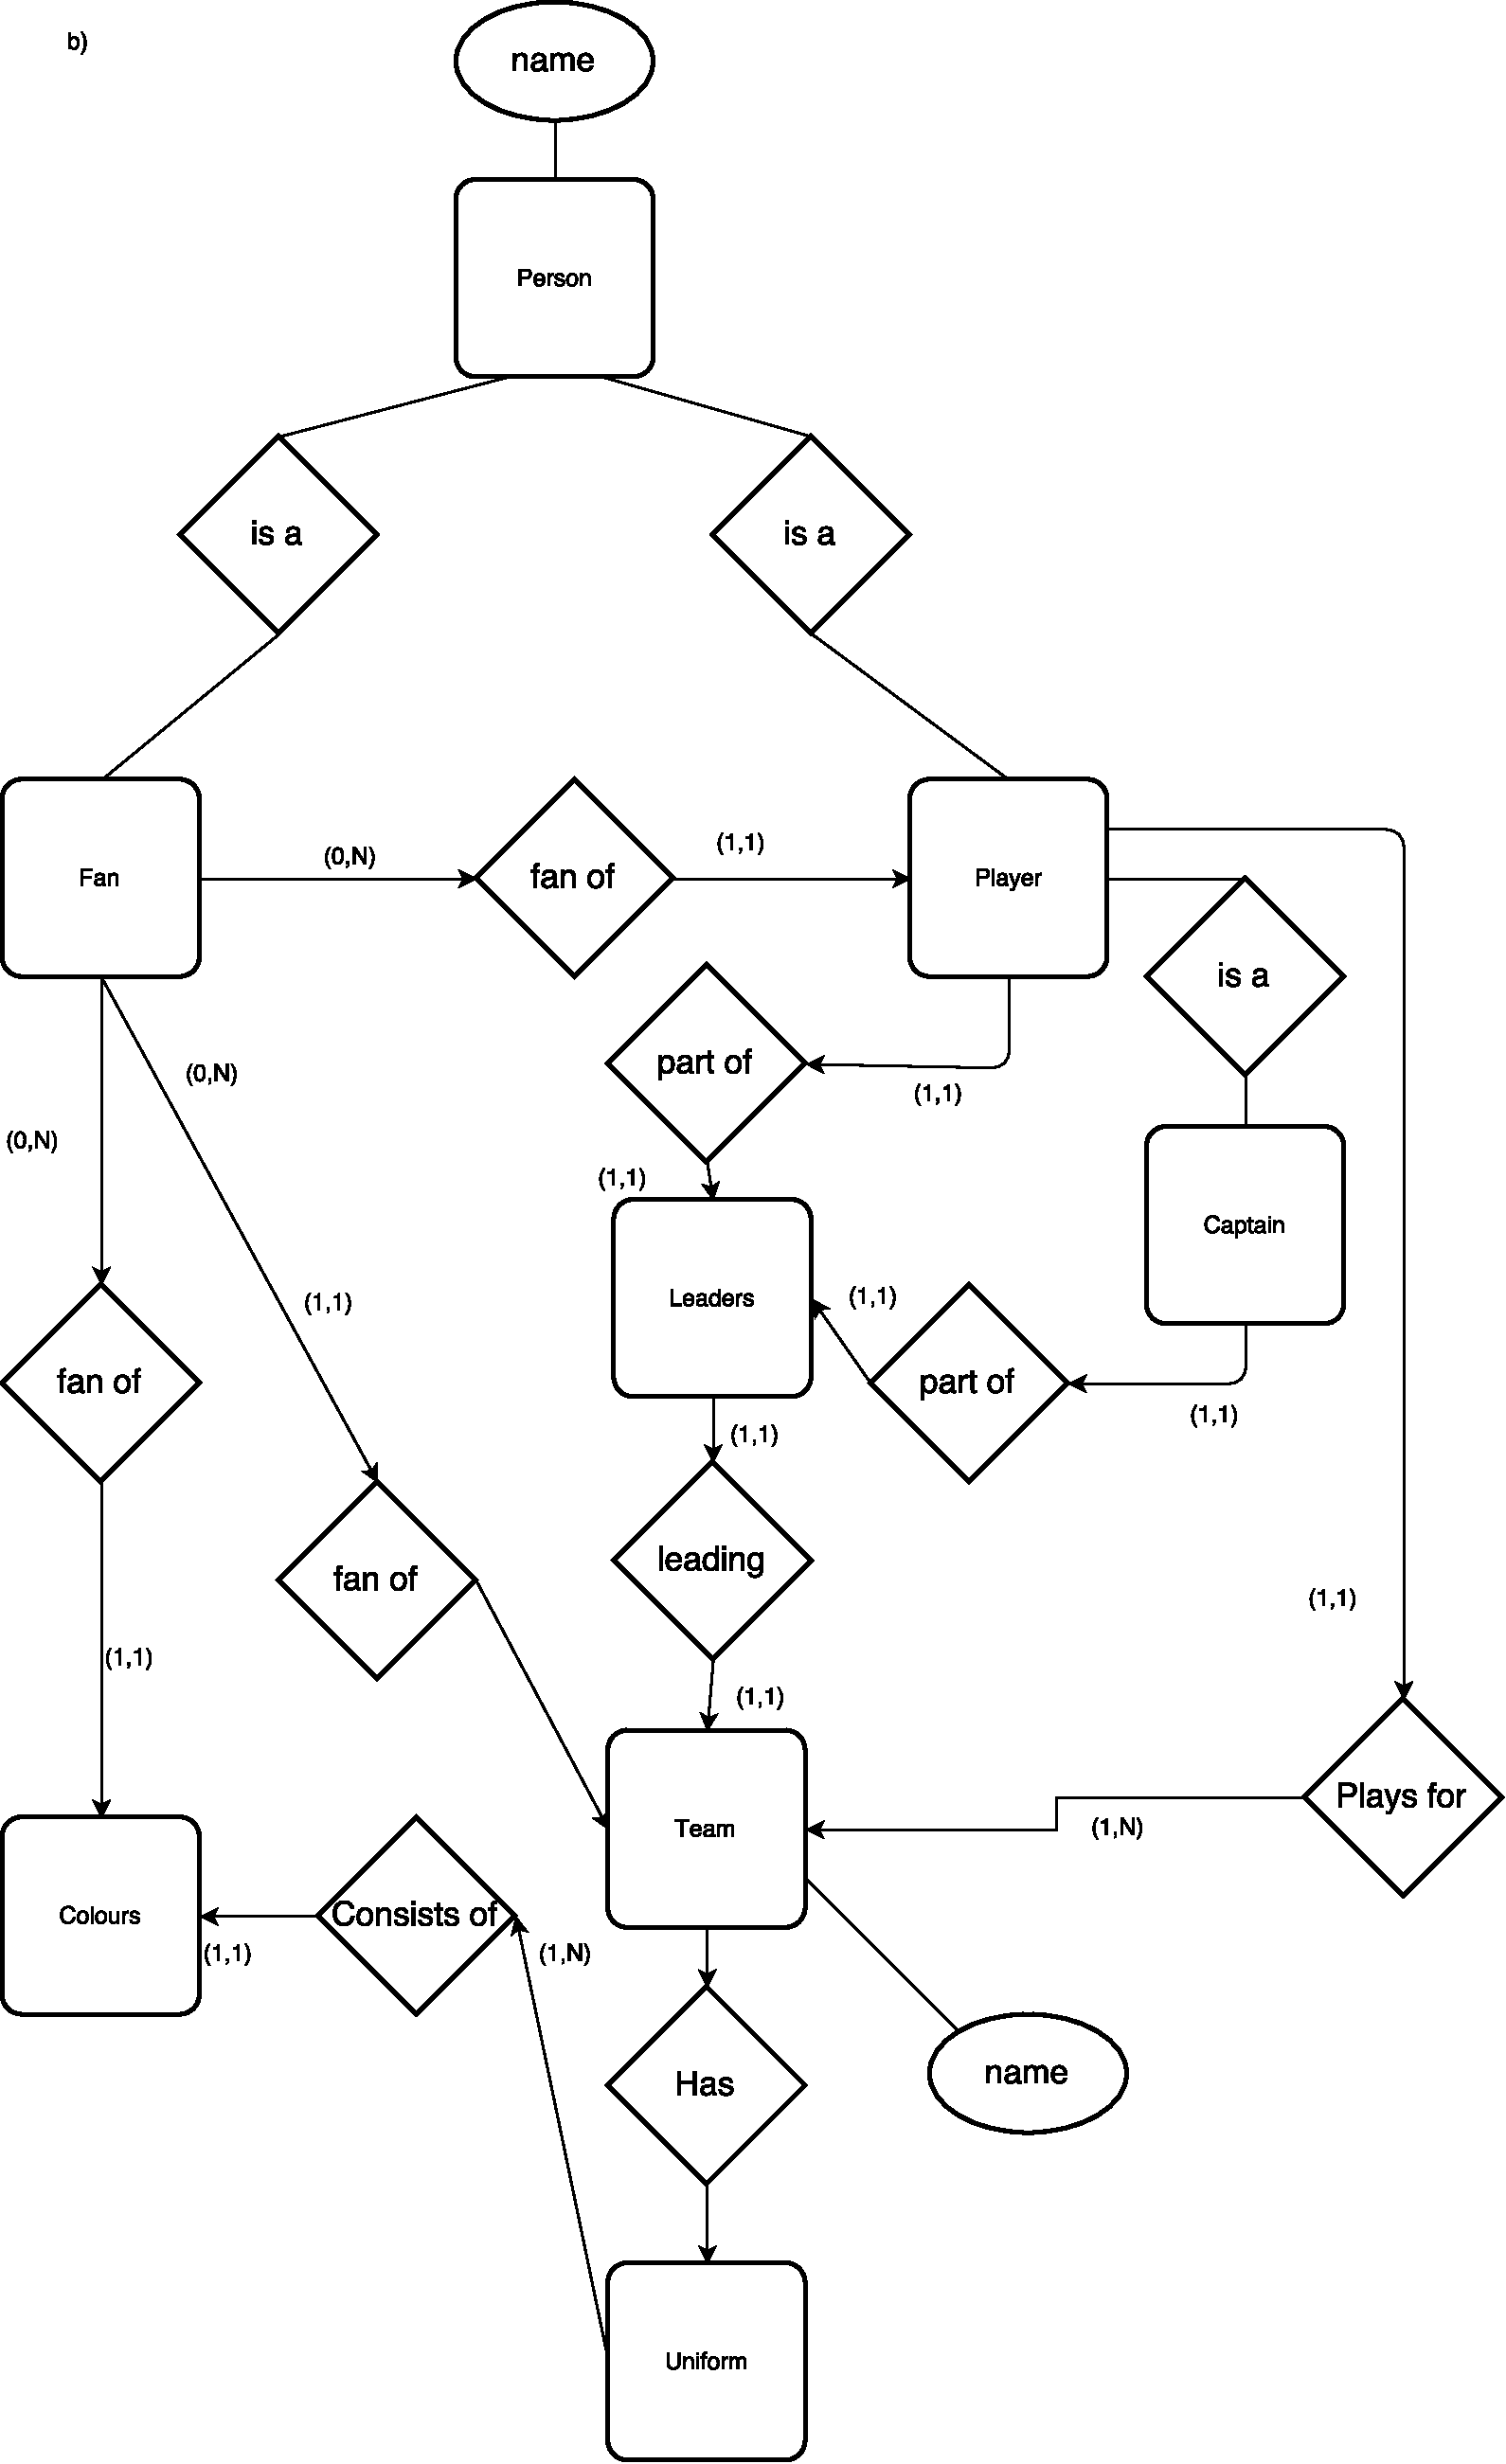
\includepdf[pages={1}]{/Users/Terence/git_repo/personal/diagrams/EX3T2P2.pdf}
       	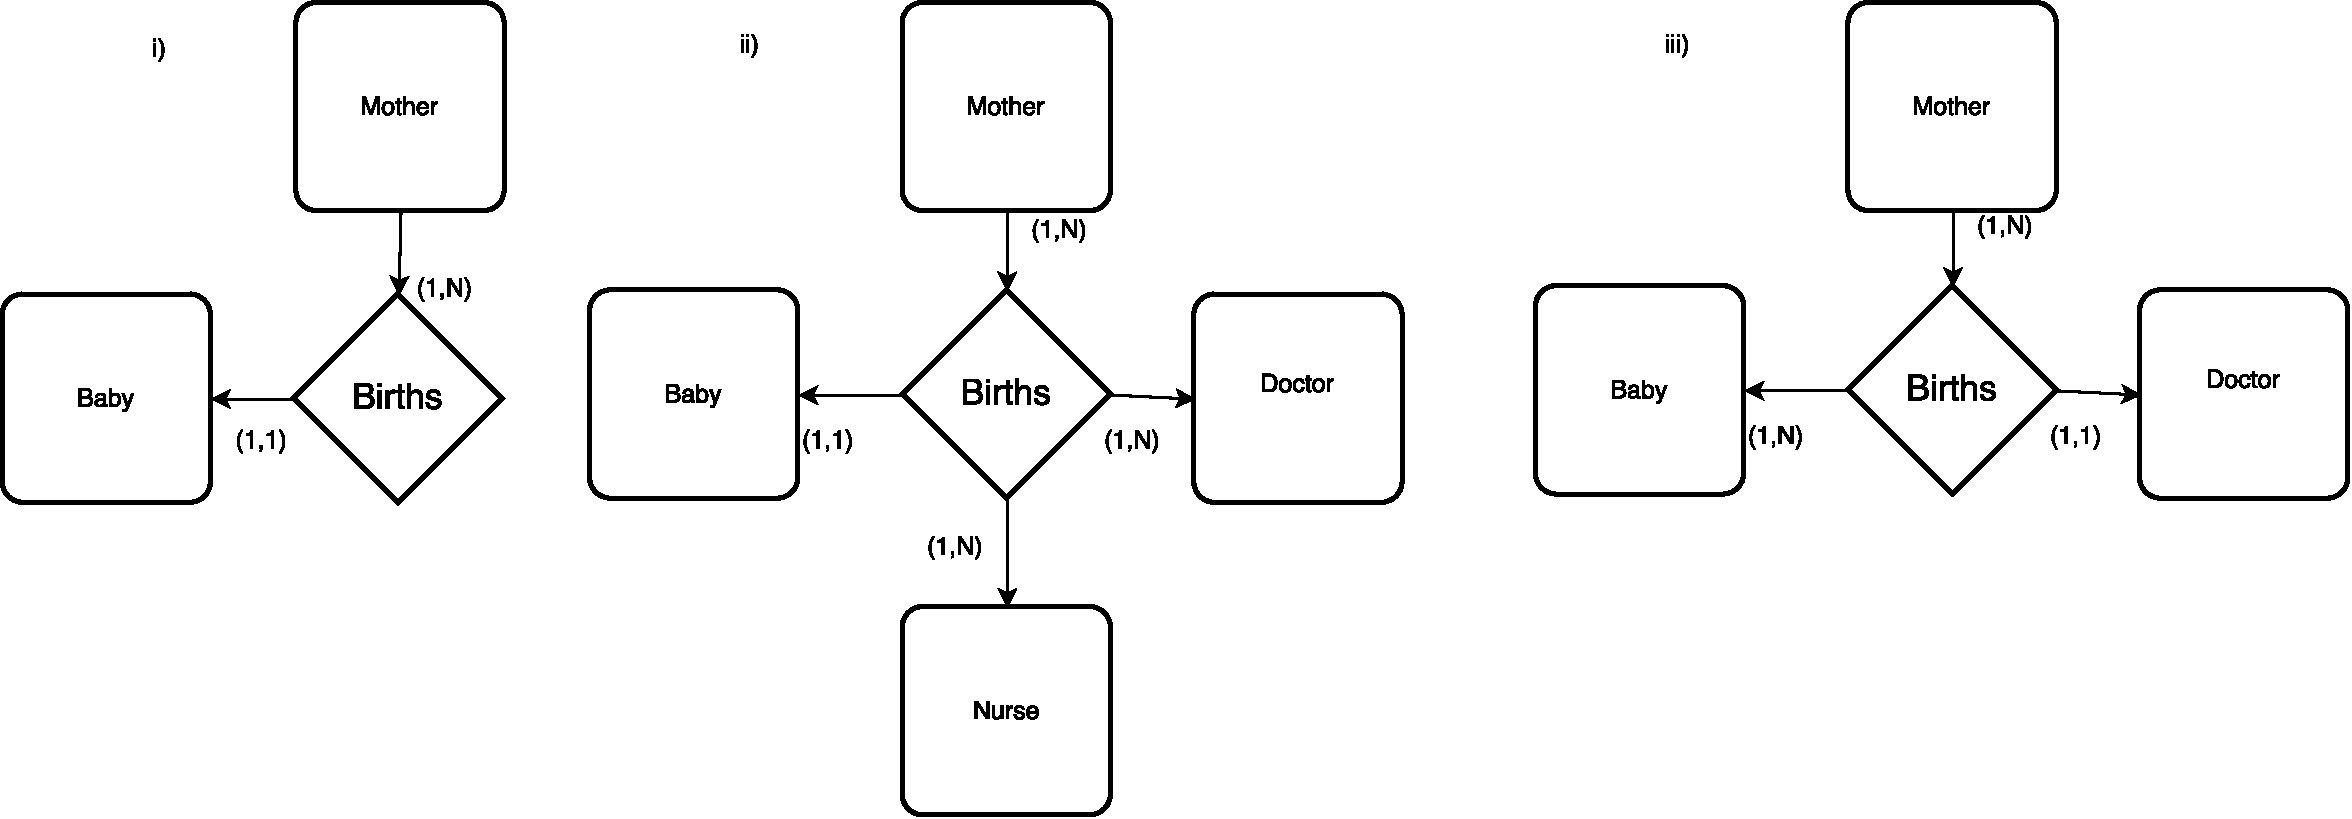
\includepdf[pages={1}]{/Users/Terence/git_repo/personal/diagrams/EX3T3P1.pdf}
       	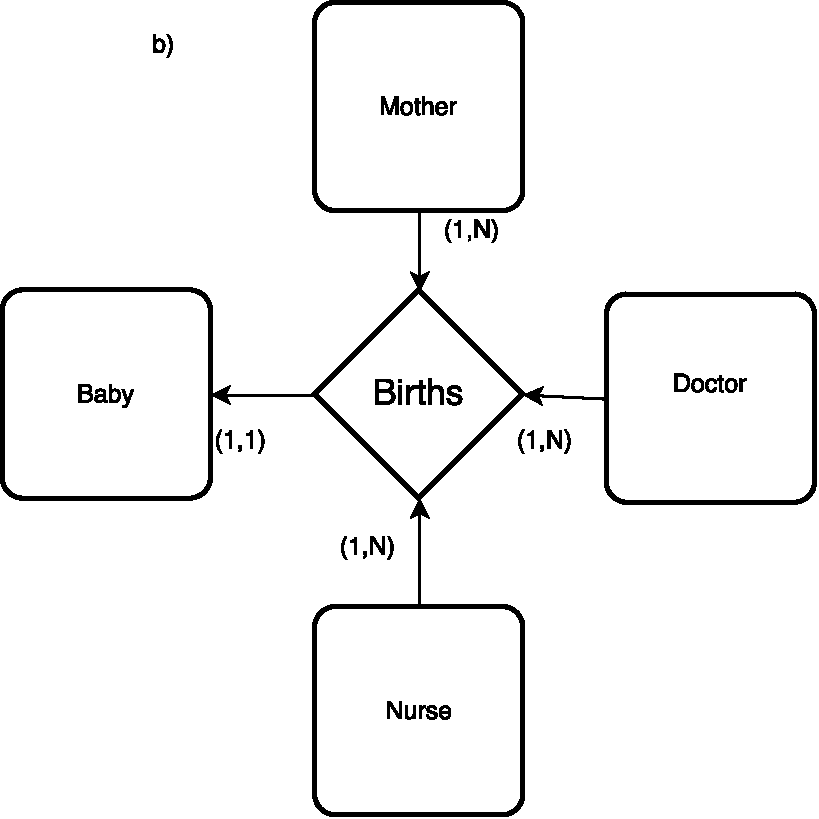
\includepdf[pages={1}]{/Users/Terence/git_repo/personal/diagrams/EX3T3P2.pdf}




       	\end{flushleft}



        \end{document}
    
    
    
    
    
    
    
